\clearpage
\section*{Experiment No.3}
\begin{figure}[h]
\begin{center}
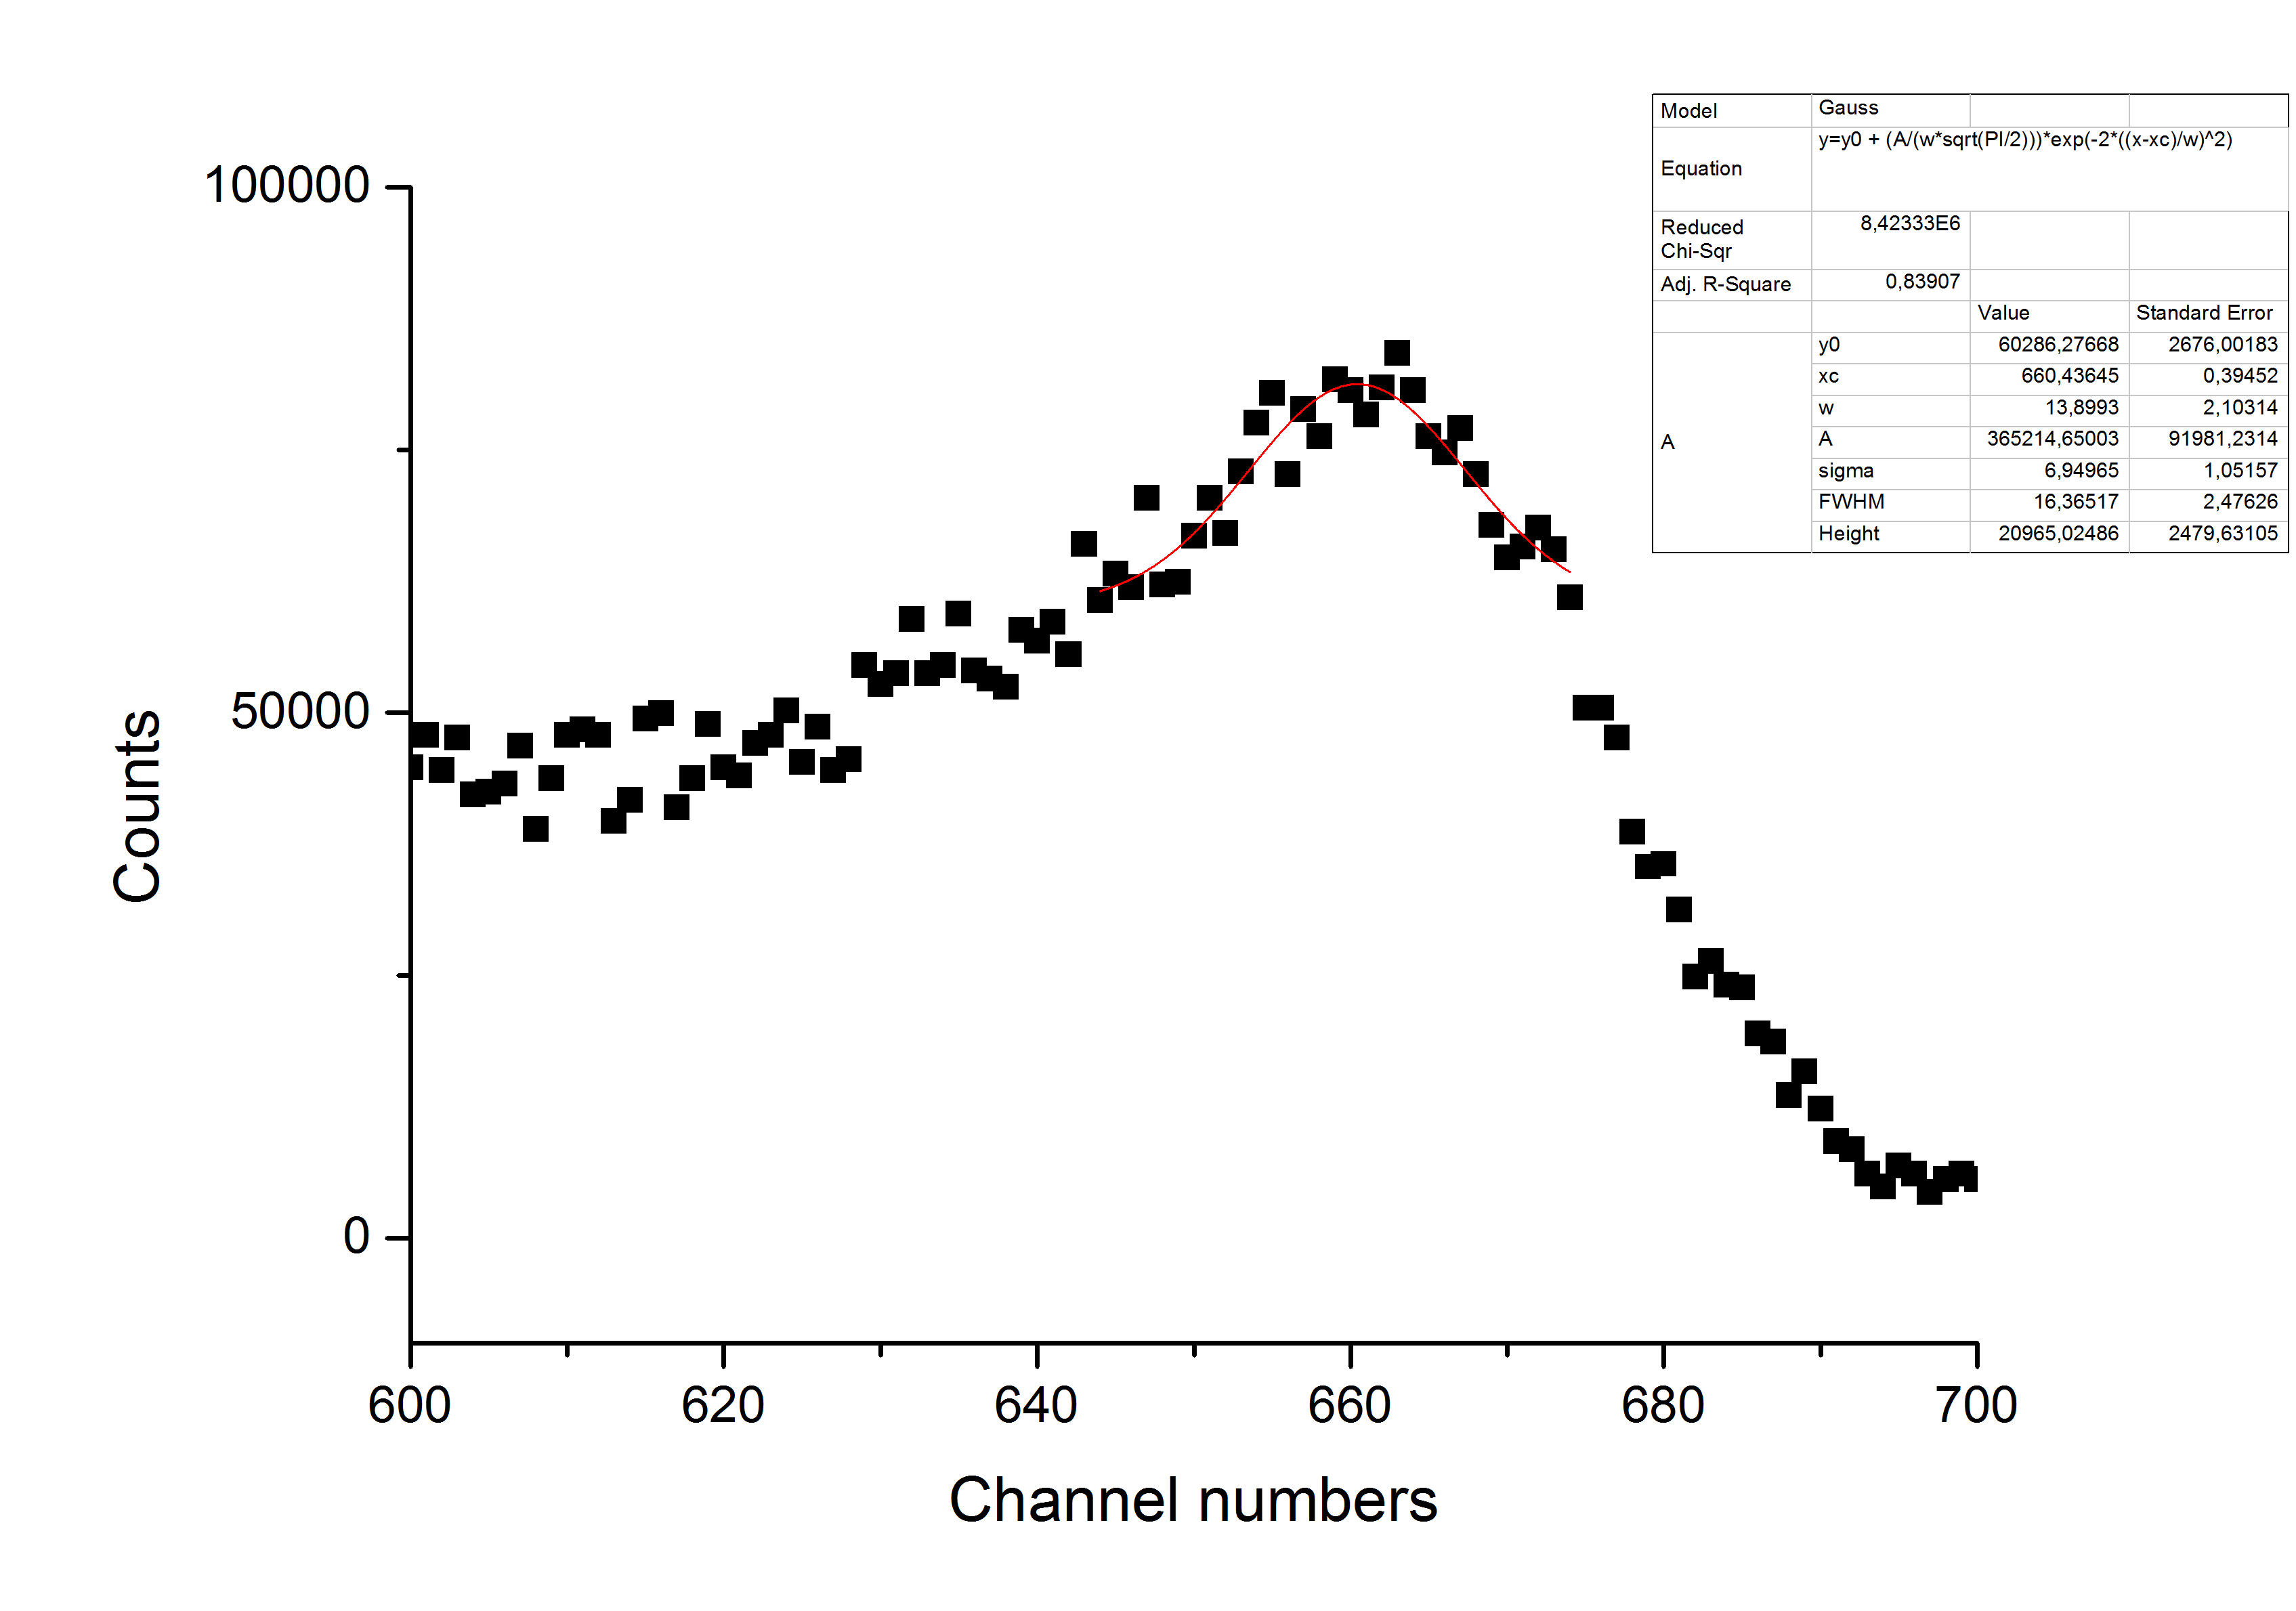
\includegraphics[scale=0.15]{Bilder/Teil3/122keV_CdTe_korrekt}
\caption{122keV, CdTe, with correction of the peak}
\label{fig:CdTeK}
\end{center}
\end{figure}
\begin{figure}[h]
\begin{center}
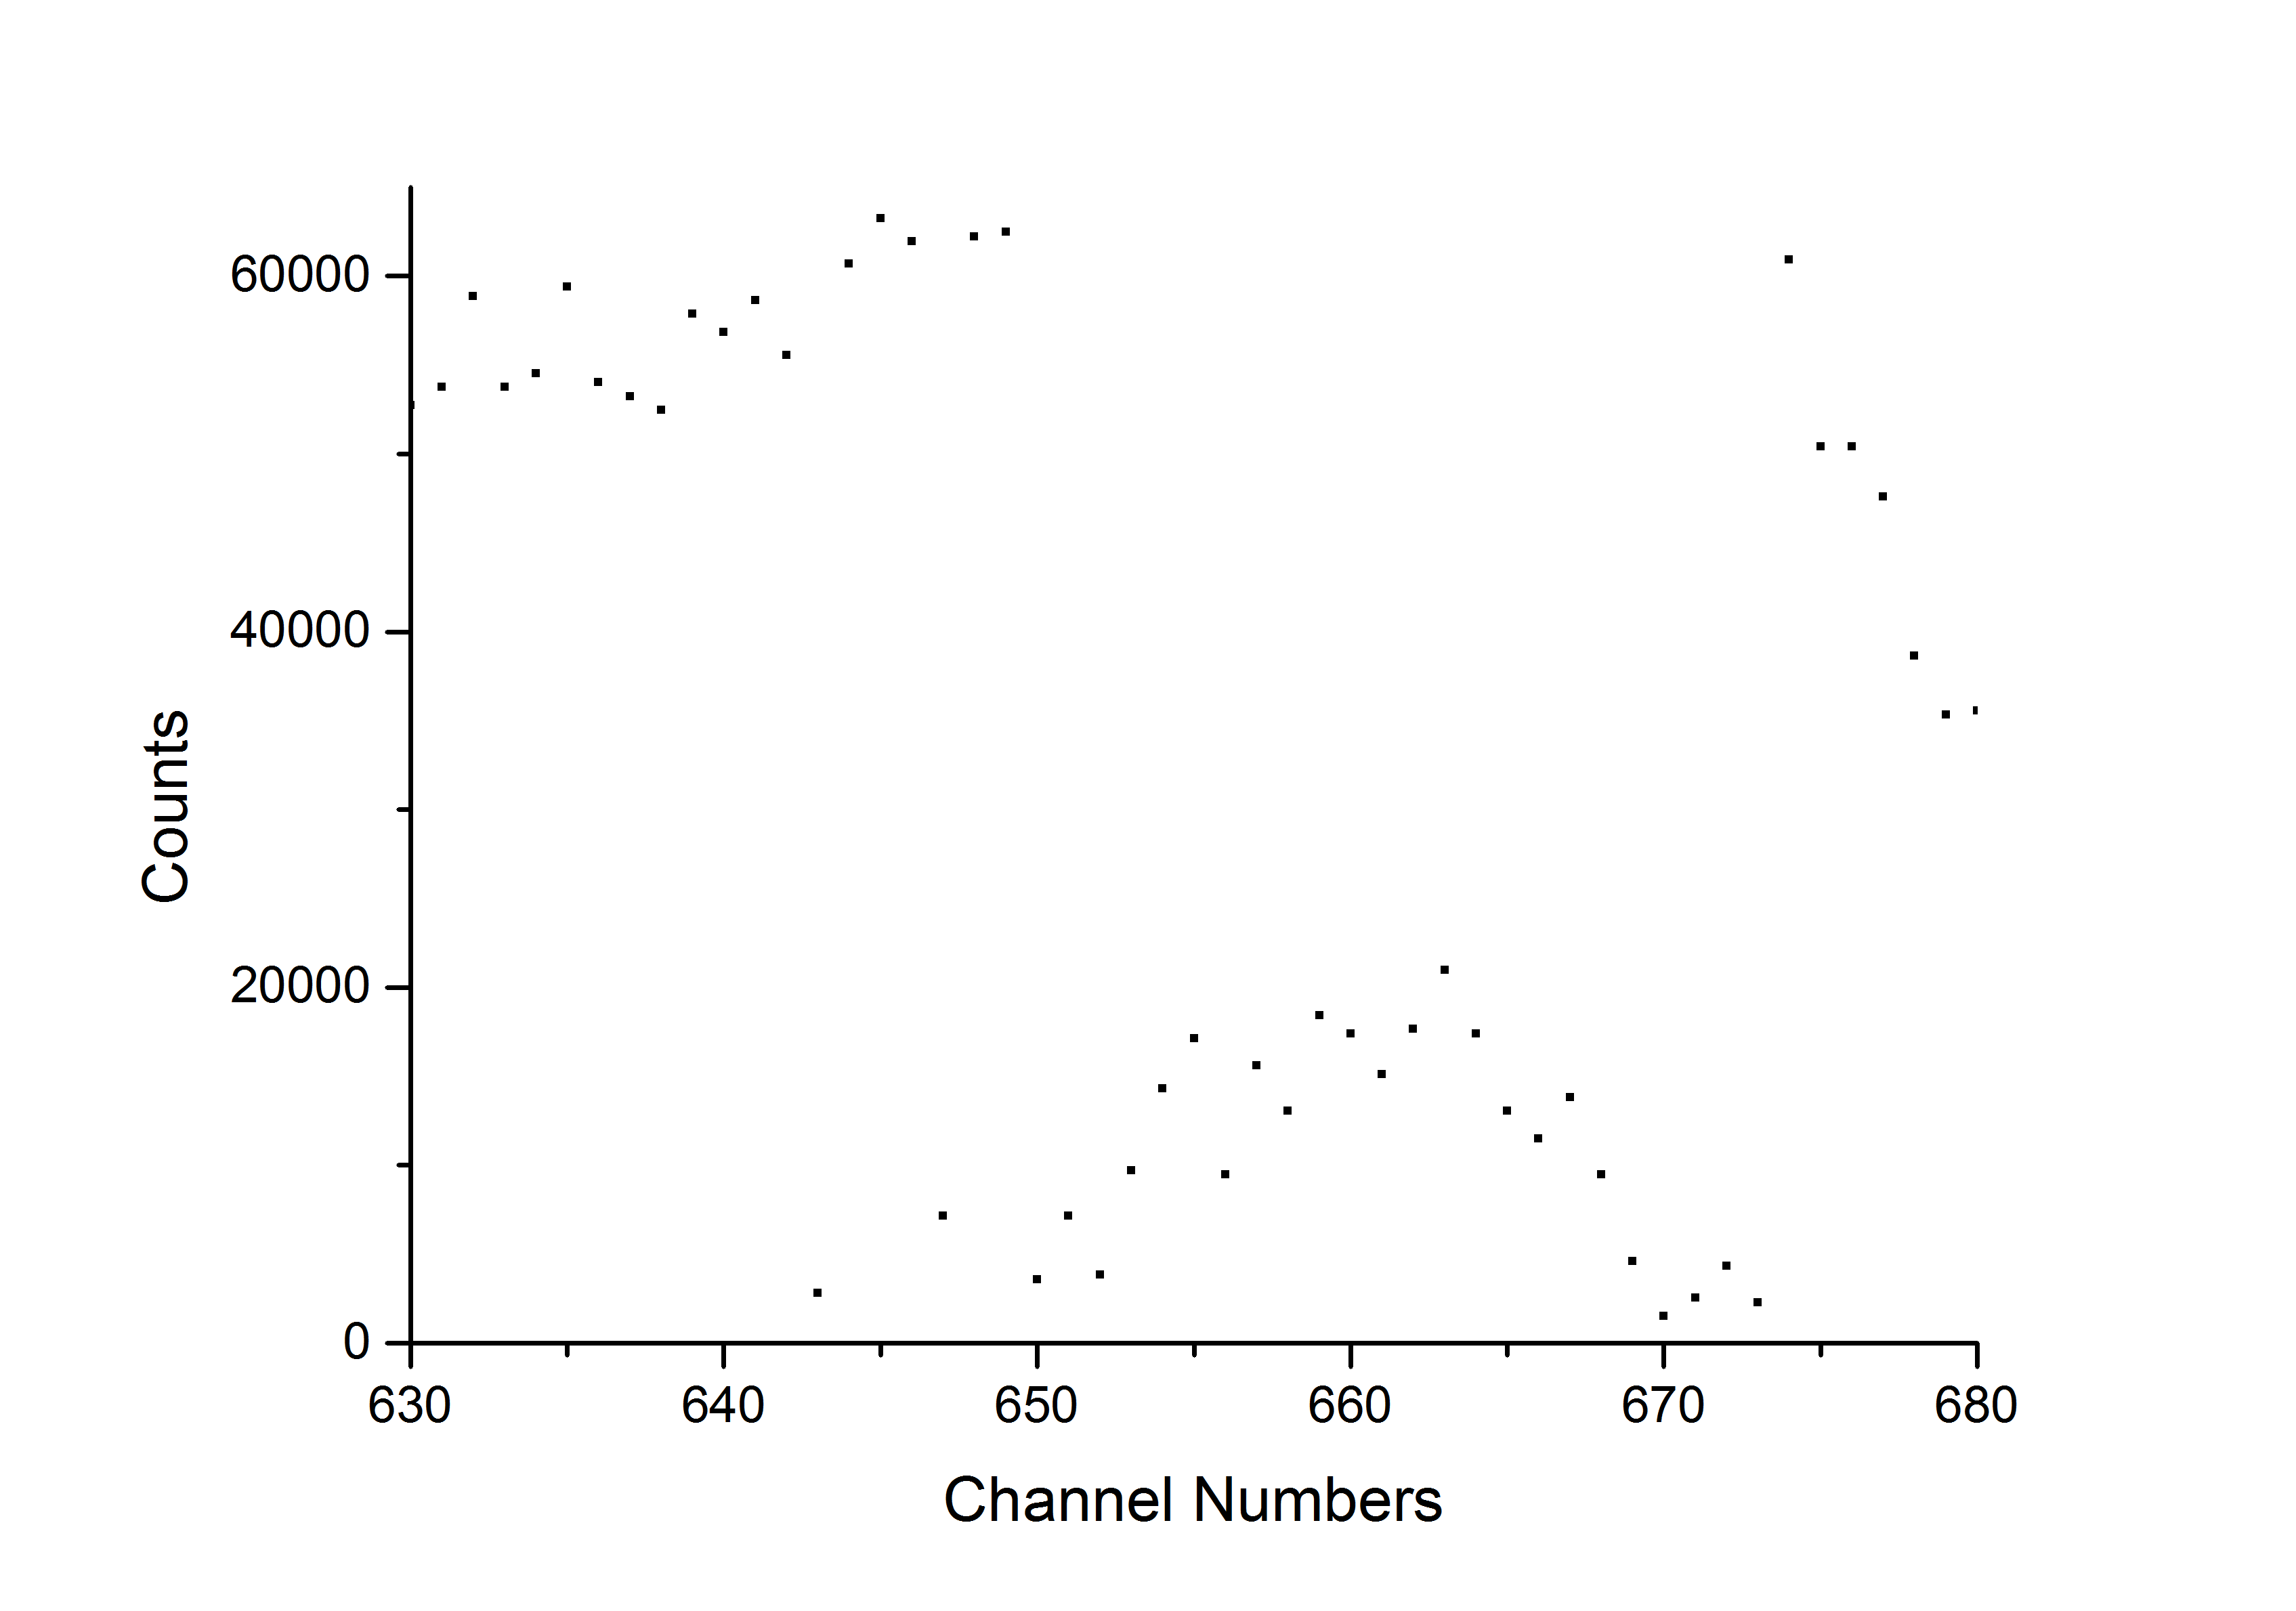
\includegraphics[scale=0.15]{Bilder/Teil3/122keV_CdTe_ohne}
\caption{122keV, CdTe, without correction of the peak}
\label{fig:CdTeO}
\end{center}
\end{figure}
\begin{figure}[h]
\begin{center}
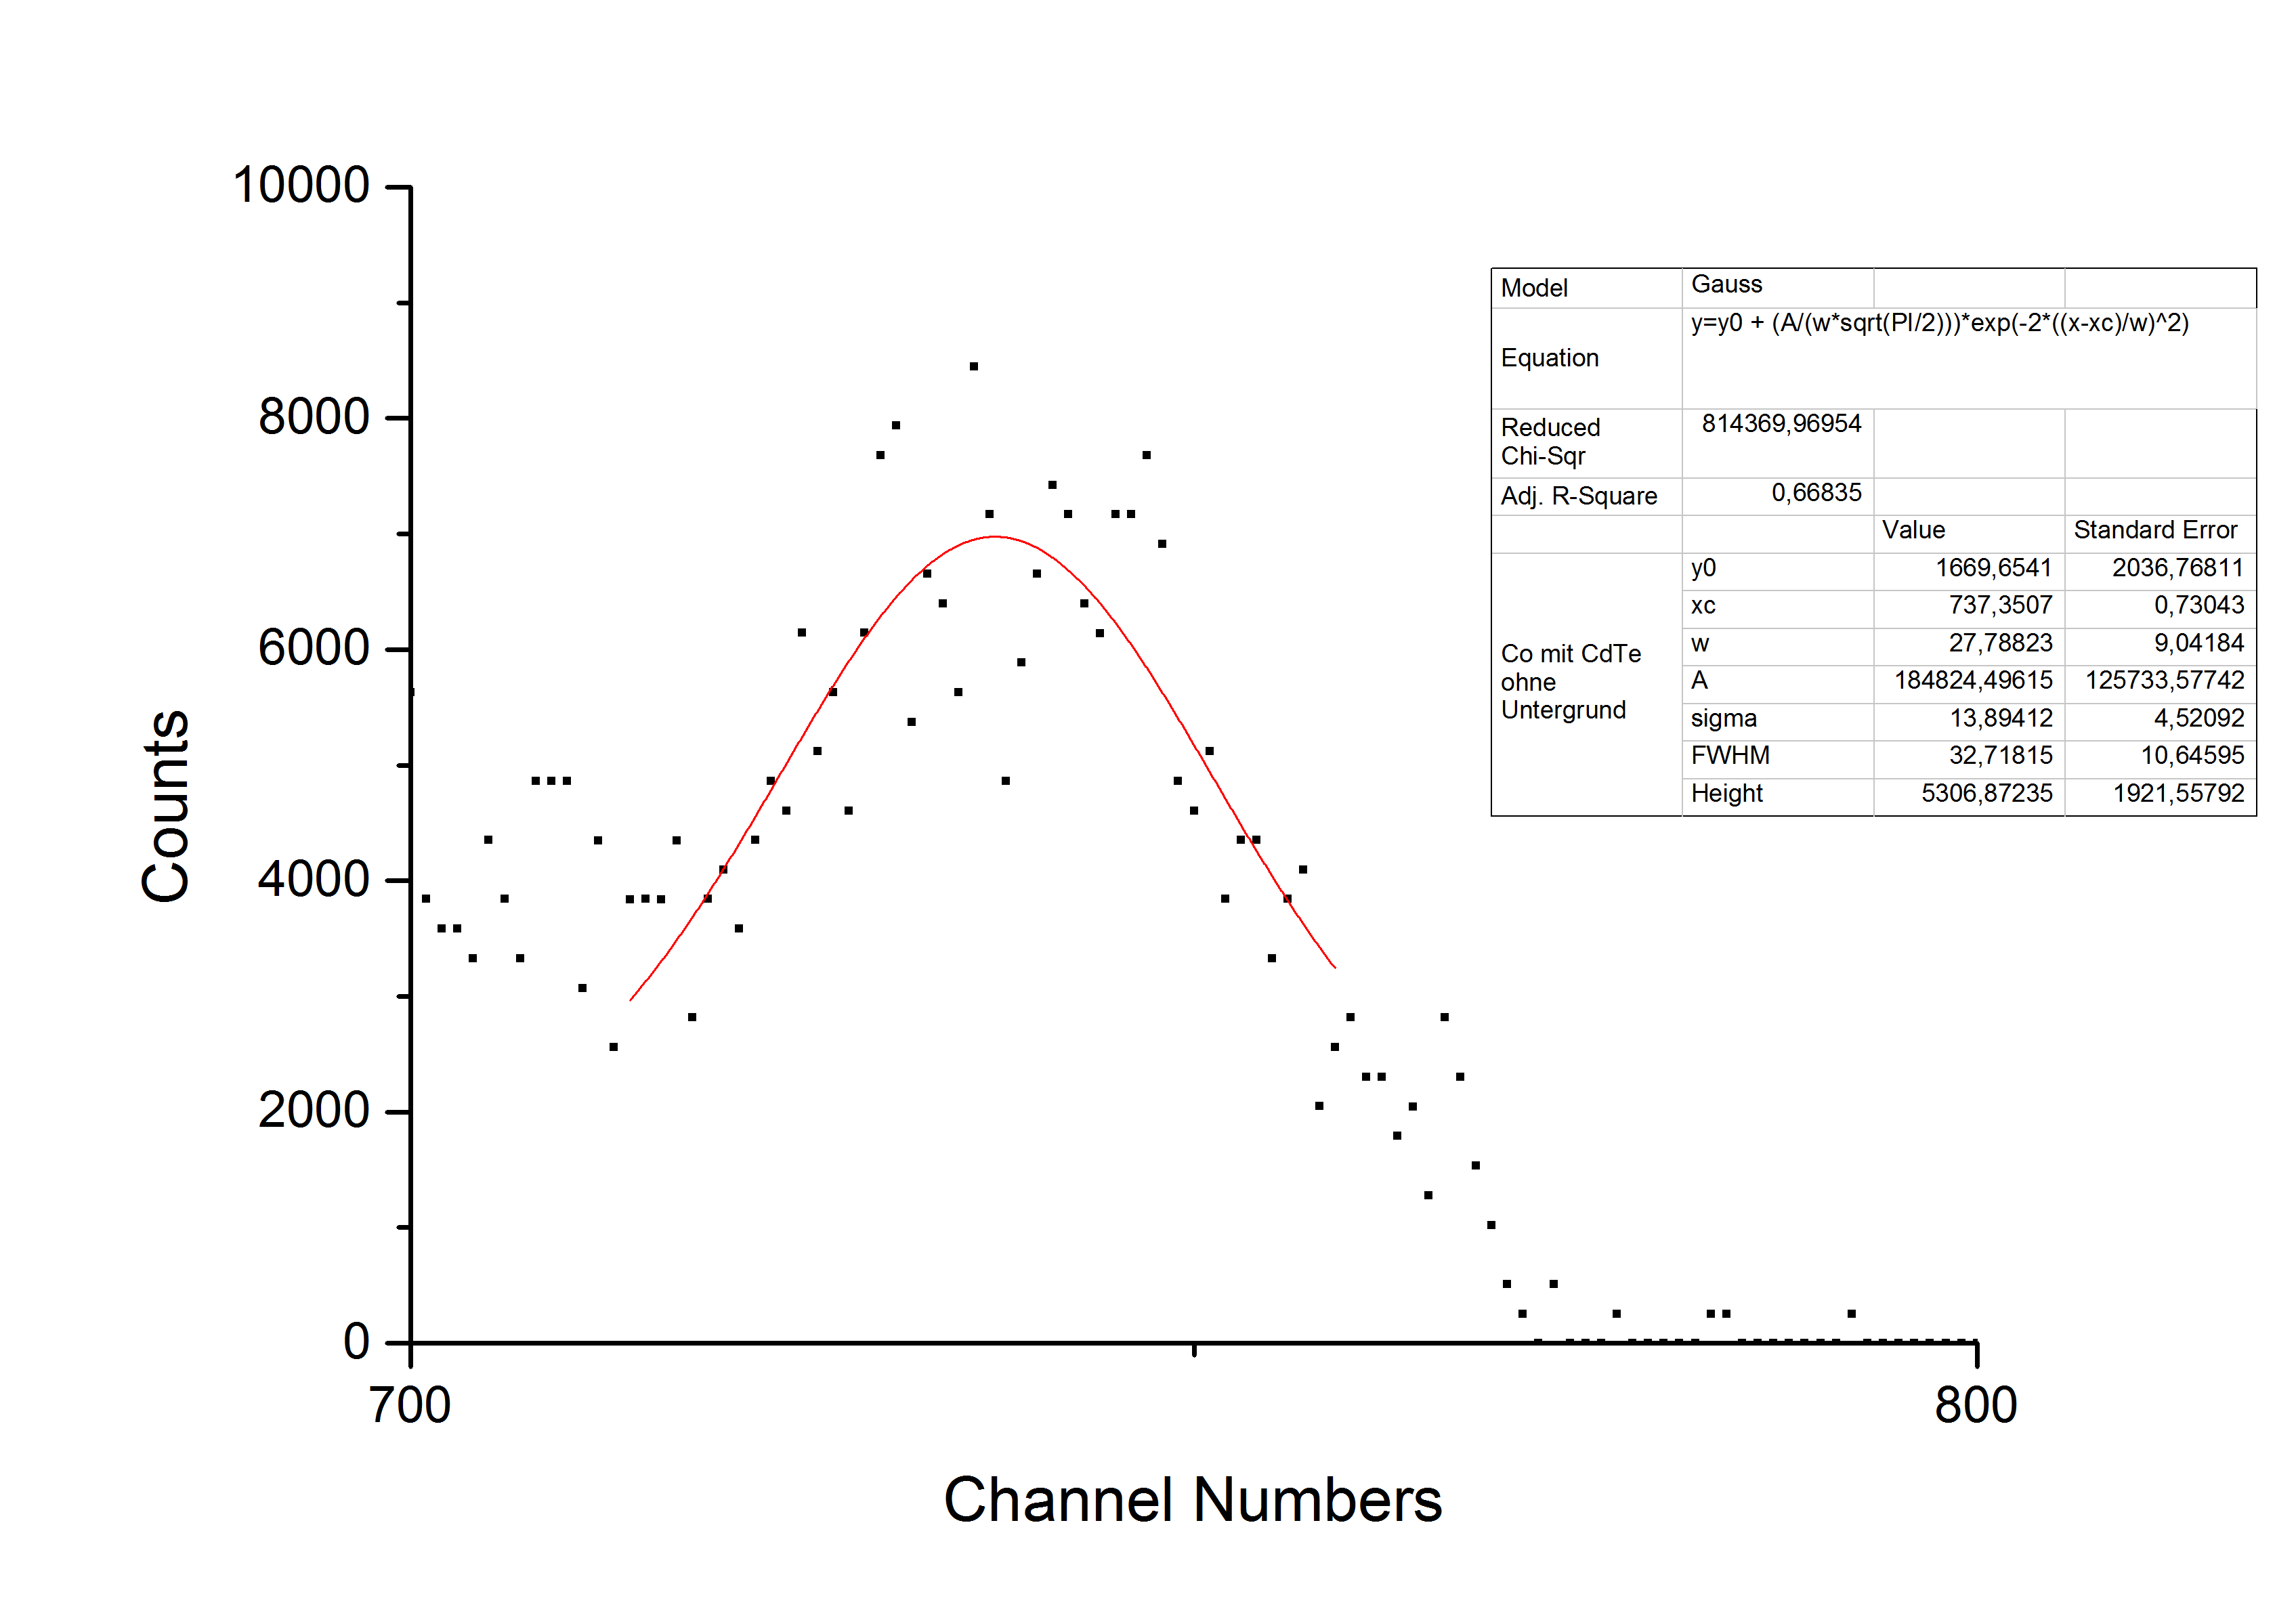
\includegraphics[scale=0.15]{Bilder/Teil3/136keV_CdTe}
\caption{136keV peak, CdTe}
\label{fig:CdTe}
\end{center}
\end{figure}
\begin{figure}[h]
\begin{center}
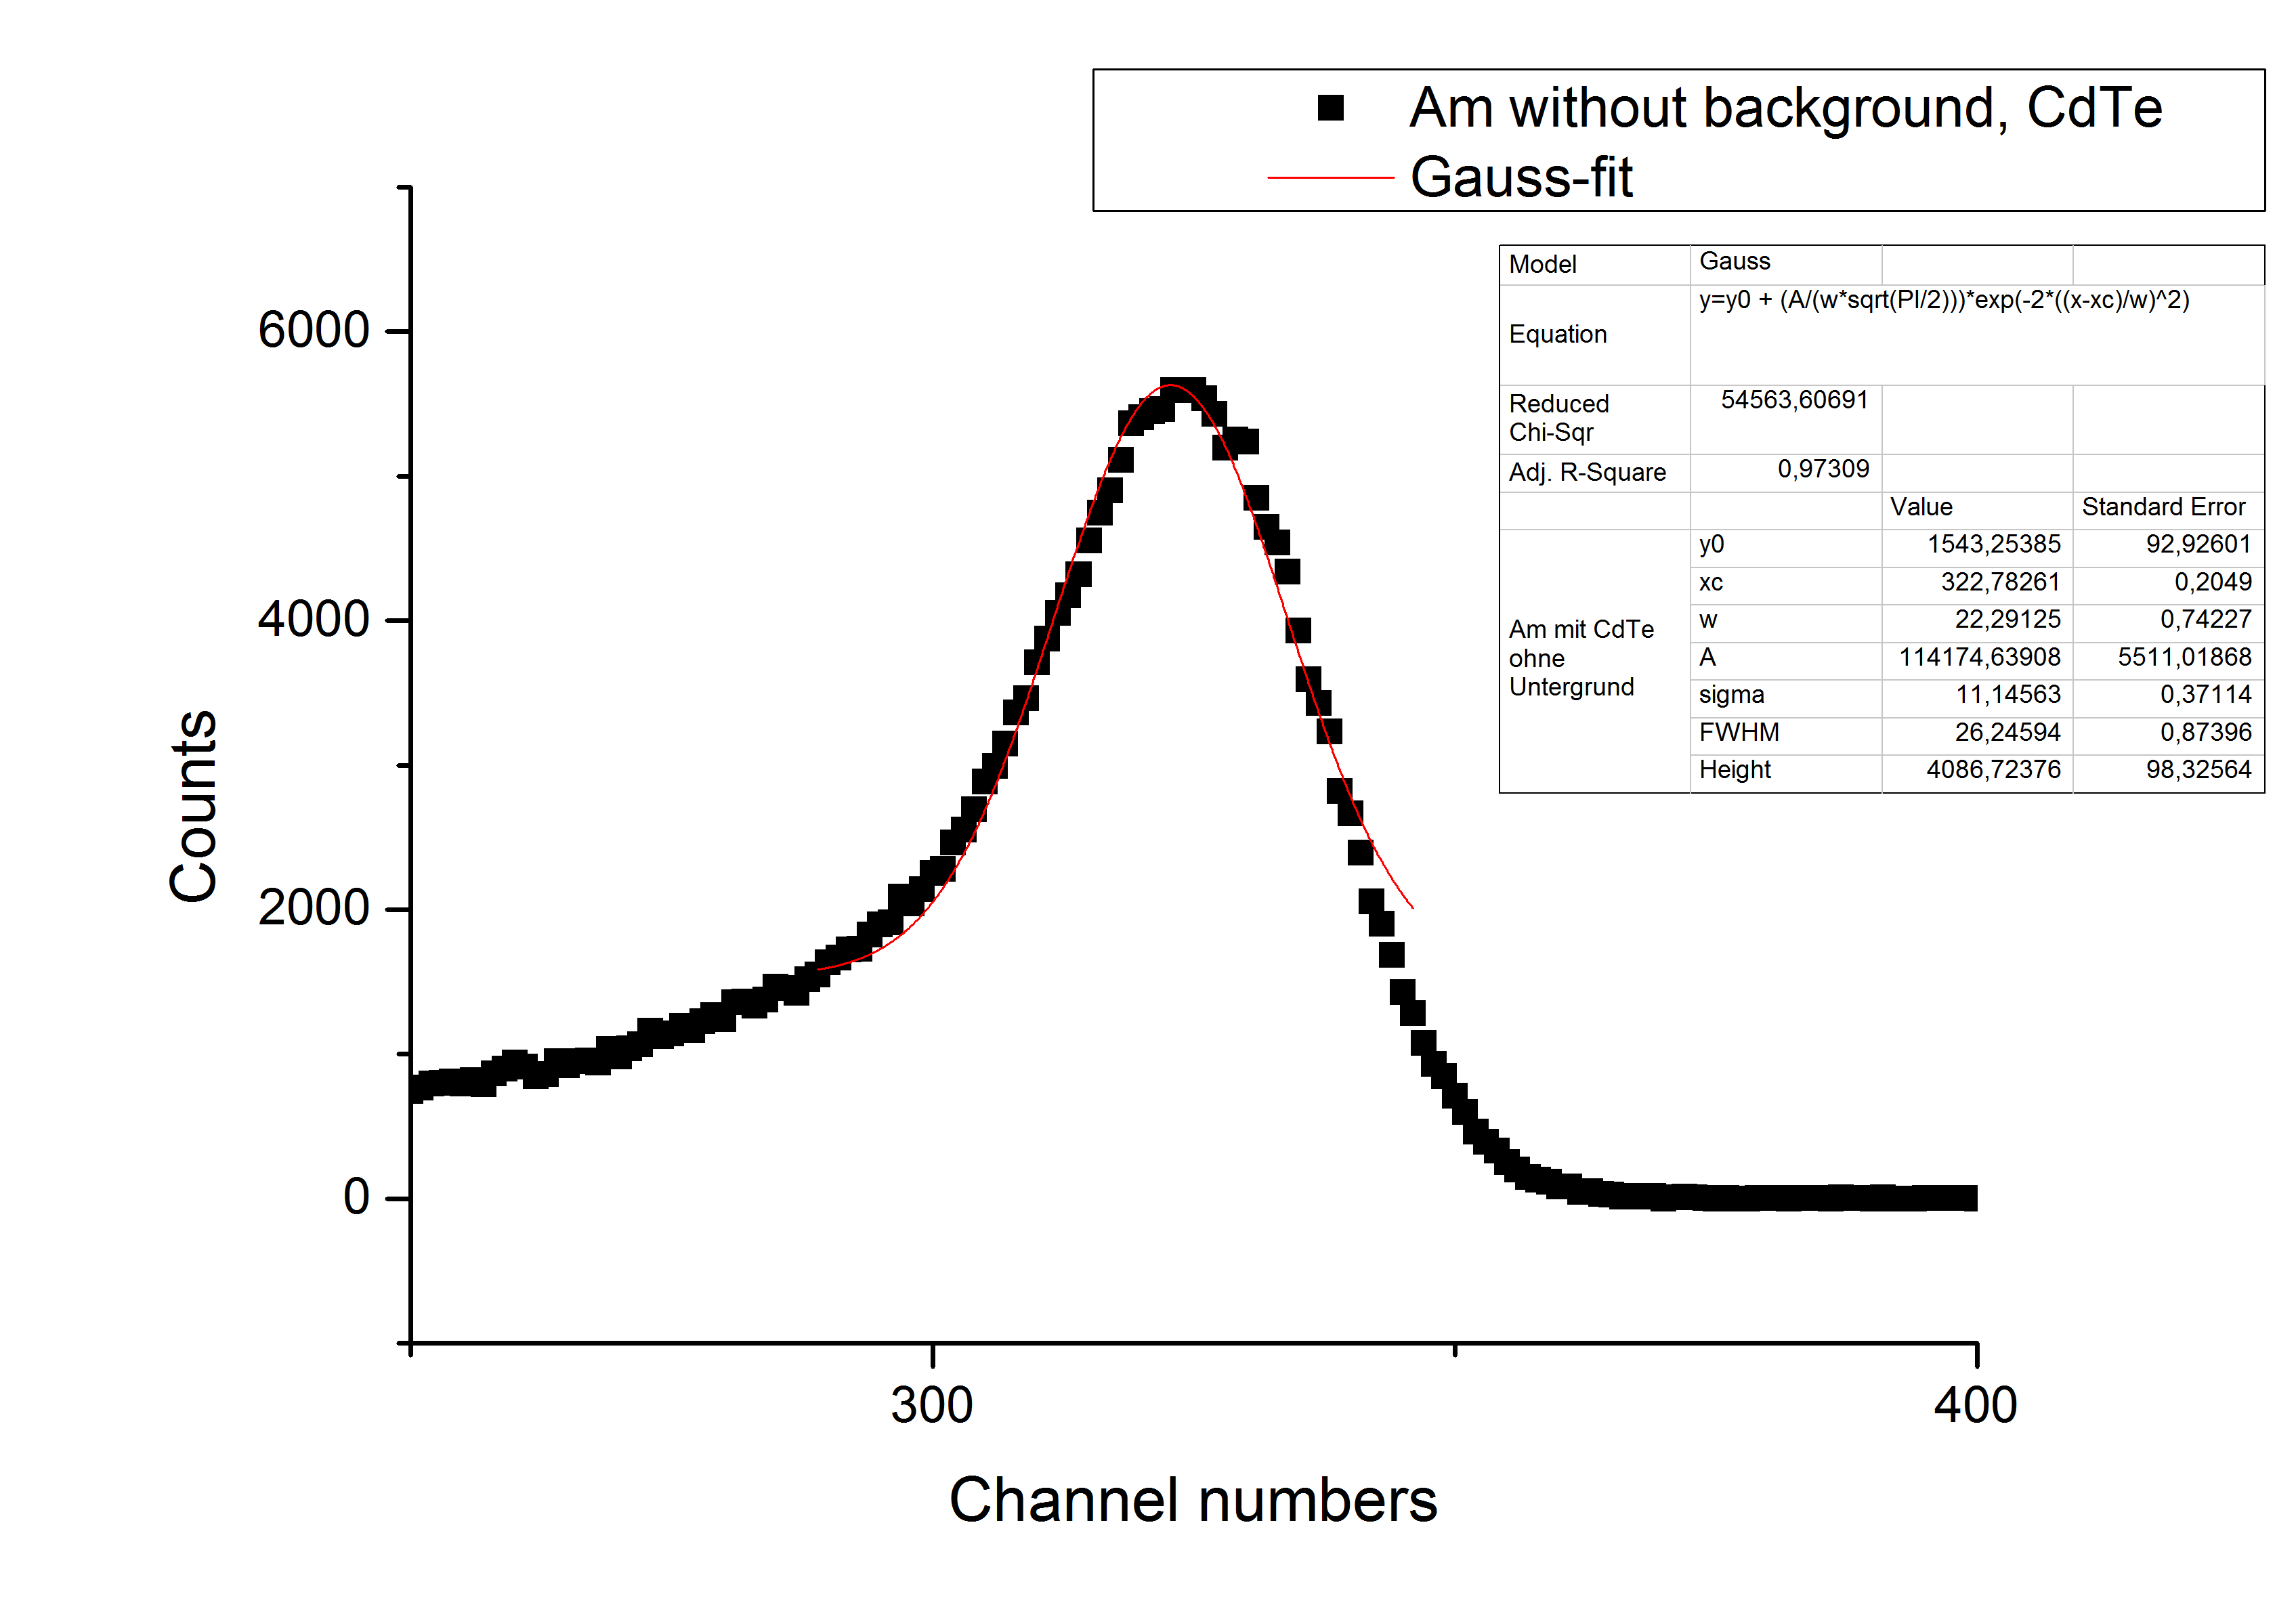
\includegraphics[scale=0.15]{Bilder/Teil3/Am_Cd}
\caption{Am with CdTe-detector}
\label{fig:AmCdTe}
\end{center}
\end{figure}
\begin{figure}[h]
\begin{center}
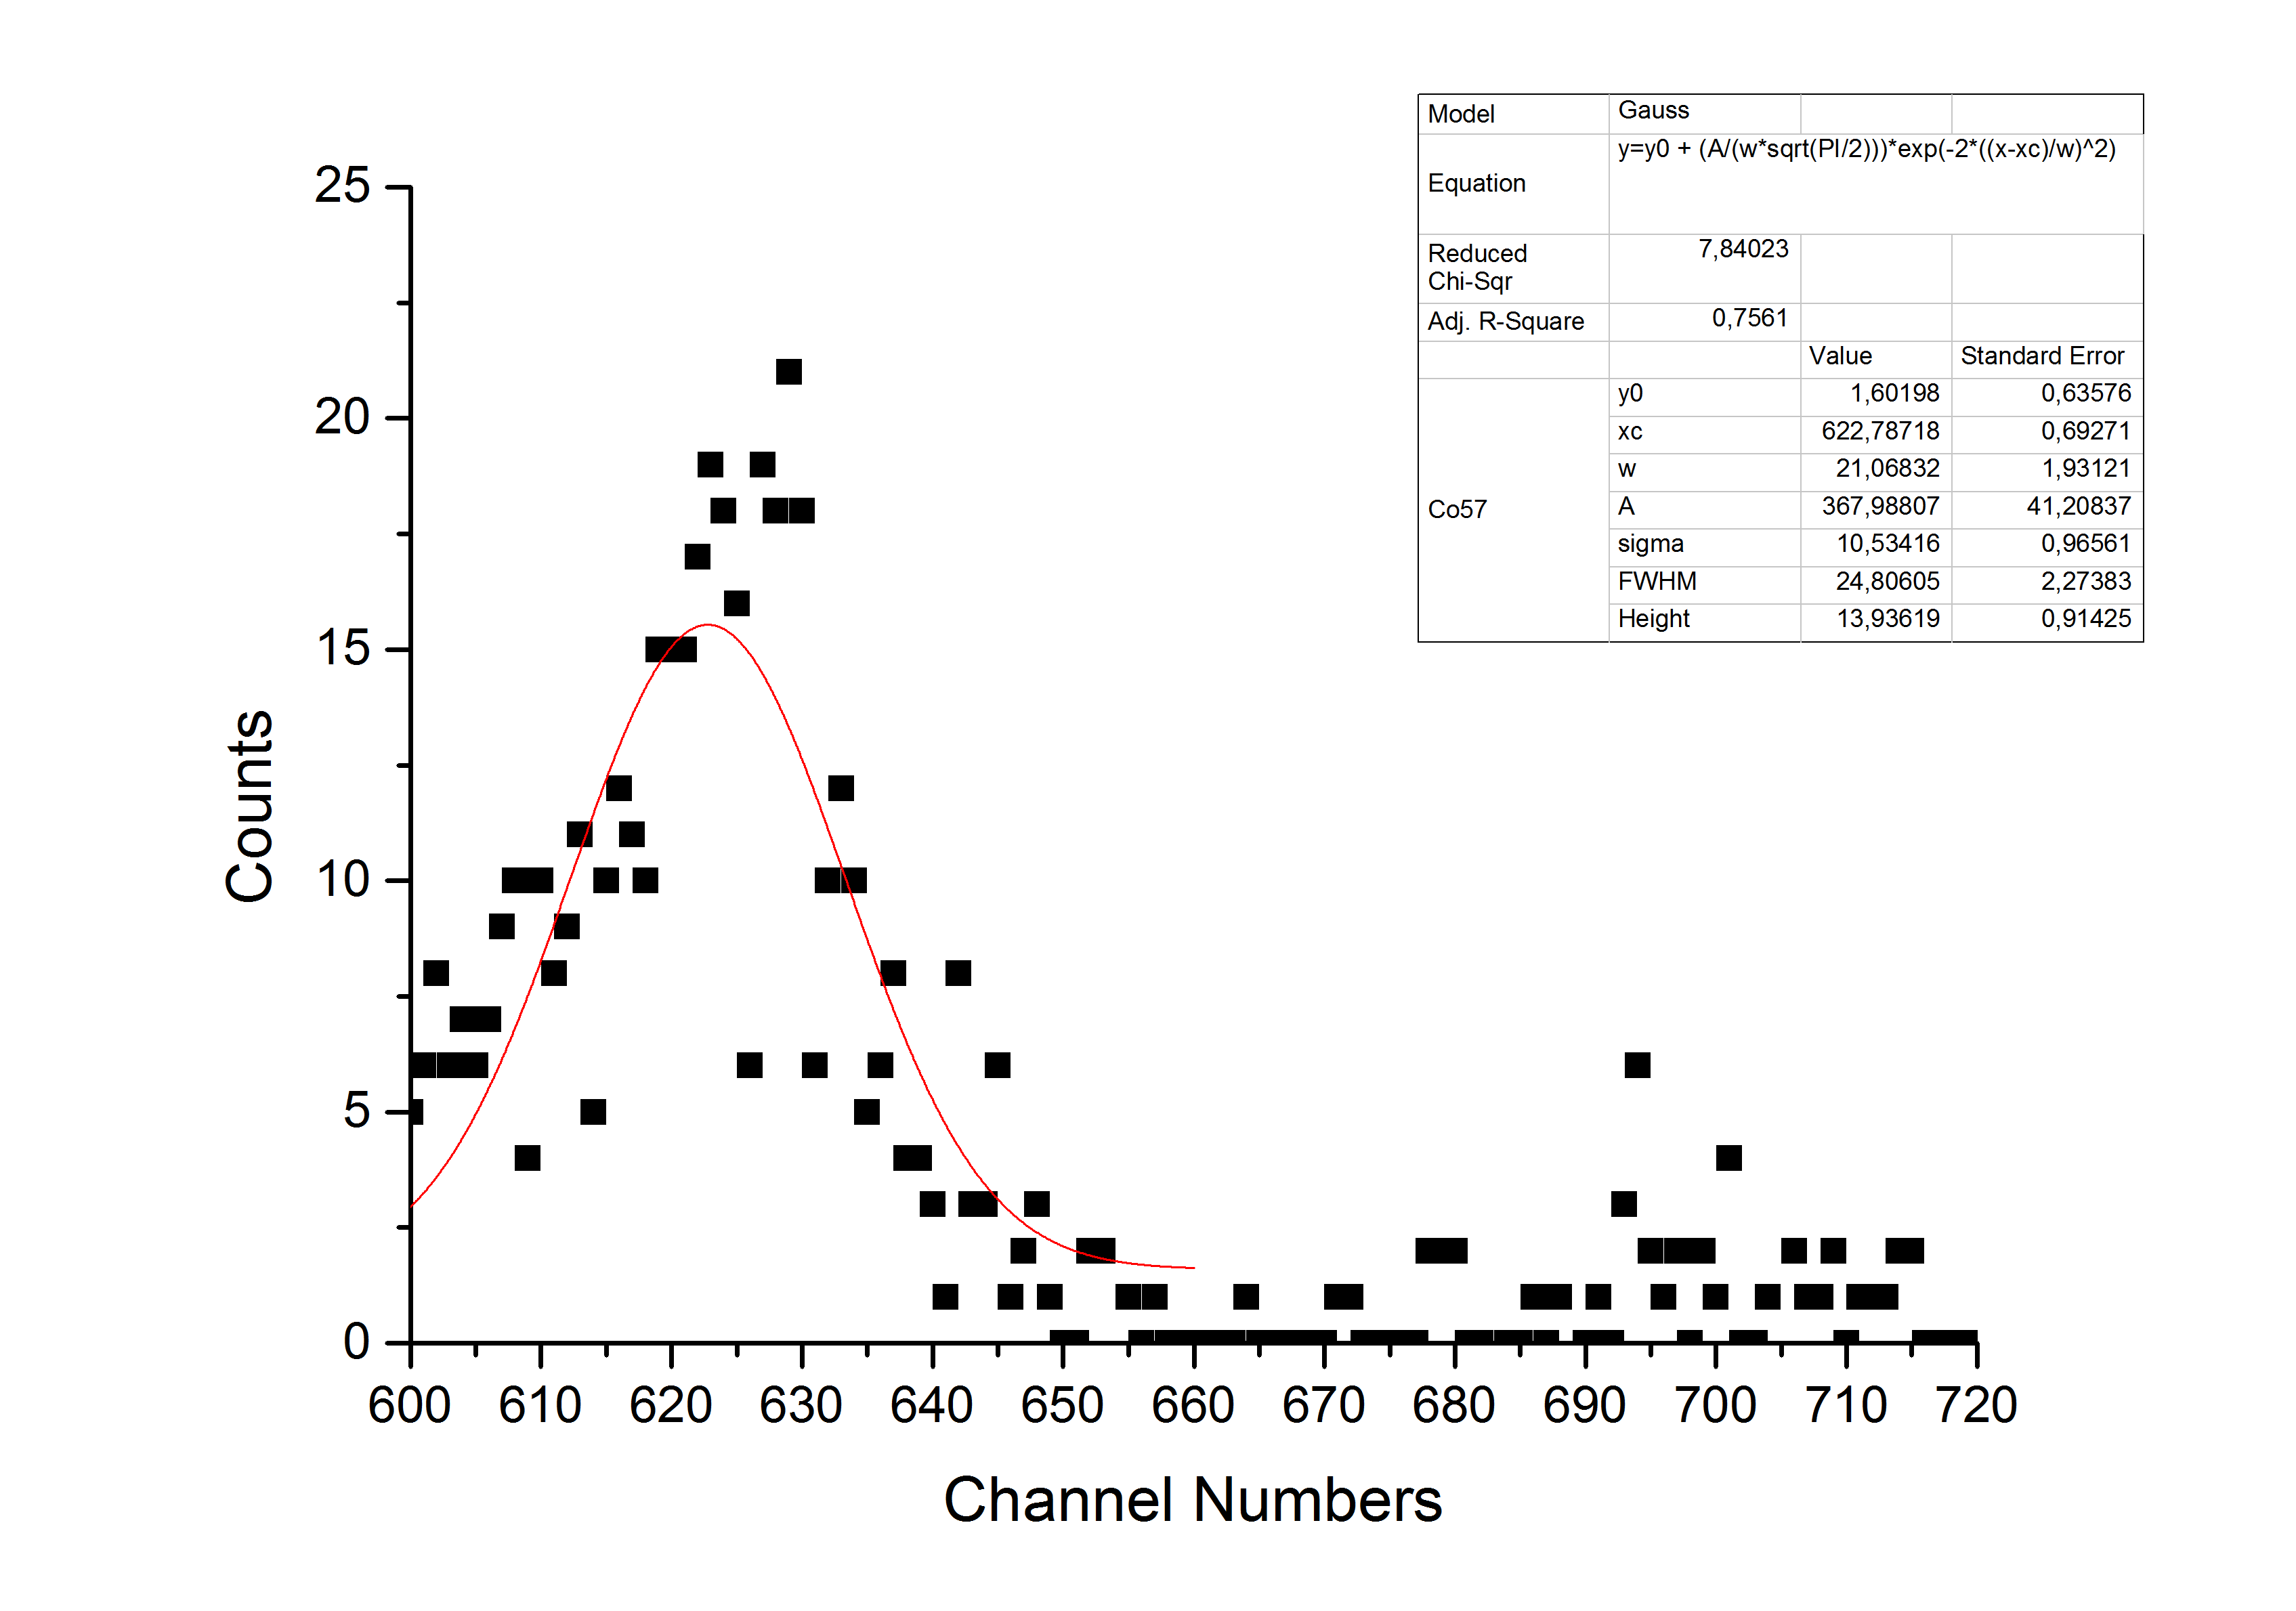
\includegraphics[scale=0.15]{Bilder/Teil3/122keV_Si}
\caption{122keV peak with Si-detector}
\label{fig:Si122}
\end{center}
\end{figure}
\begin{figure}[h]
\begin{center}
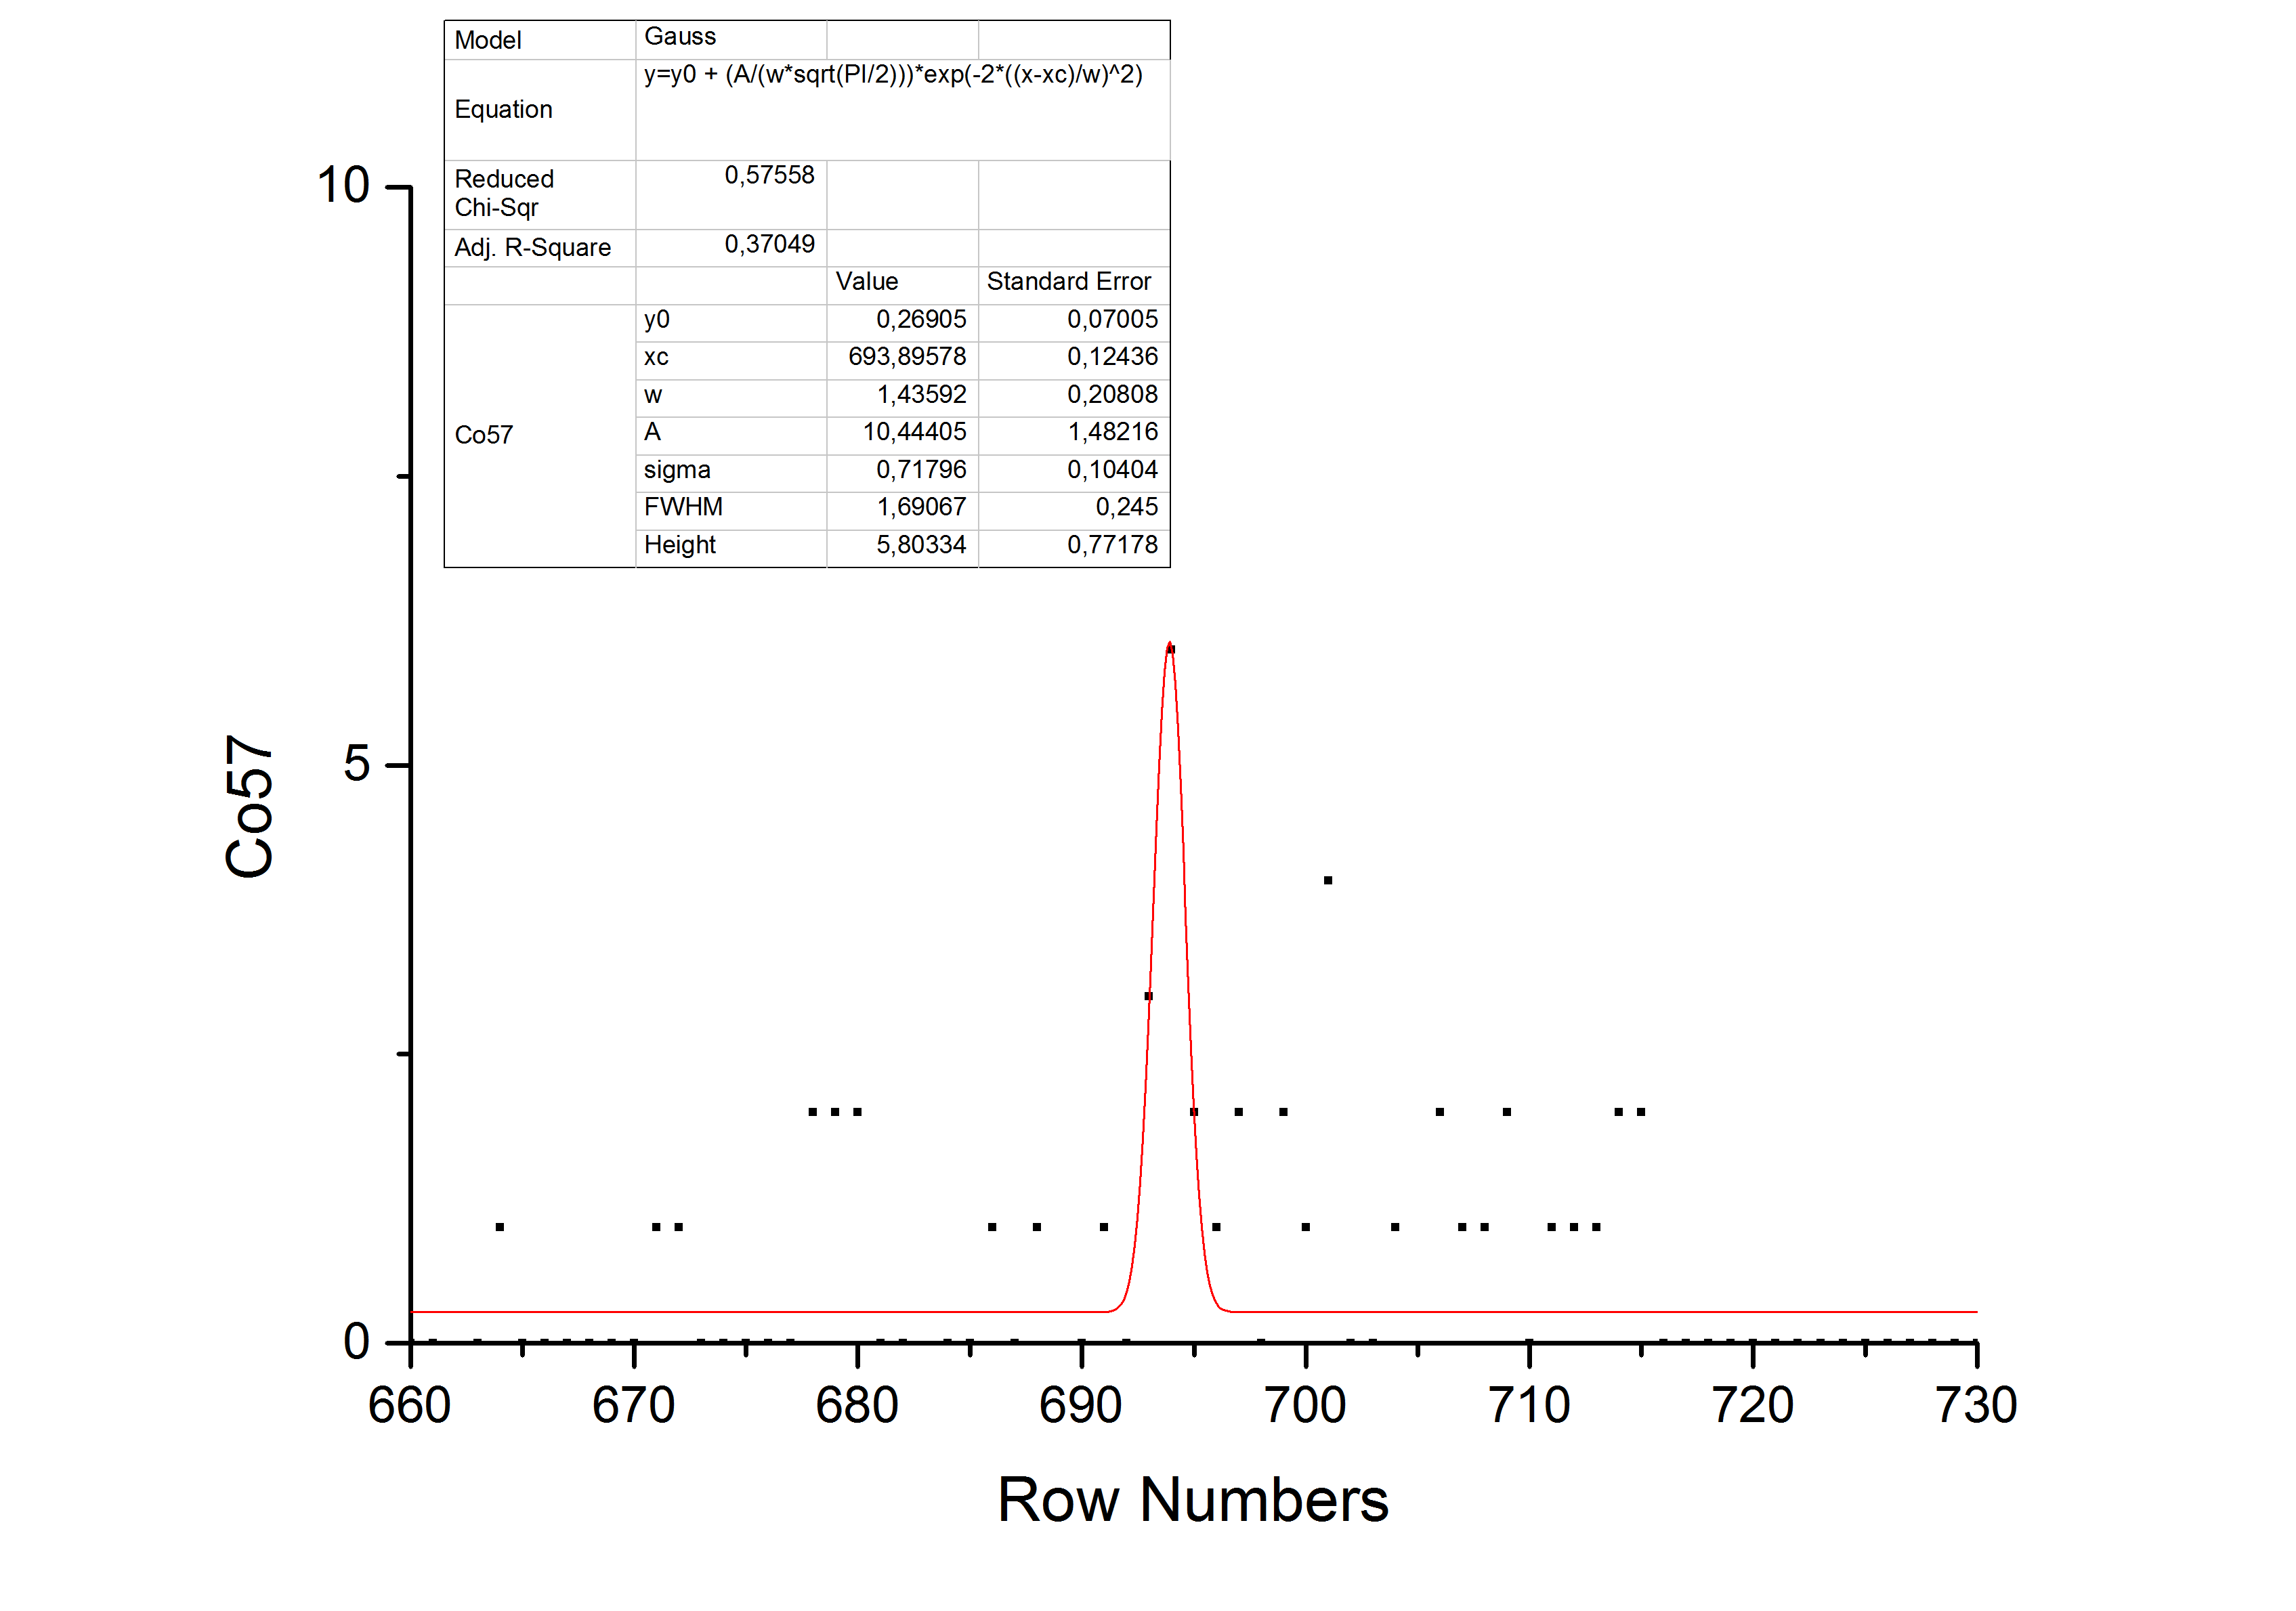
\includegraphics[scale=0.15]{Bilder/Teil3/136keV_Si}
\caption{136keV peak with Si-detector}
\label{fig:Si136}
\end{center}
\end{figure}
\begin{figure}[h]
\begin{center}
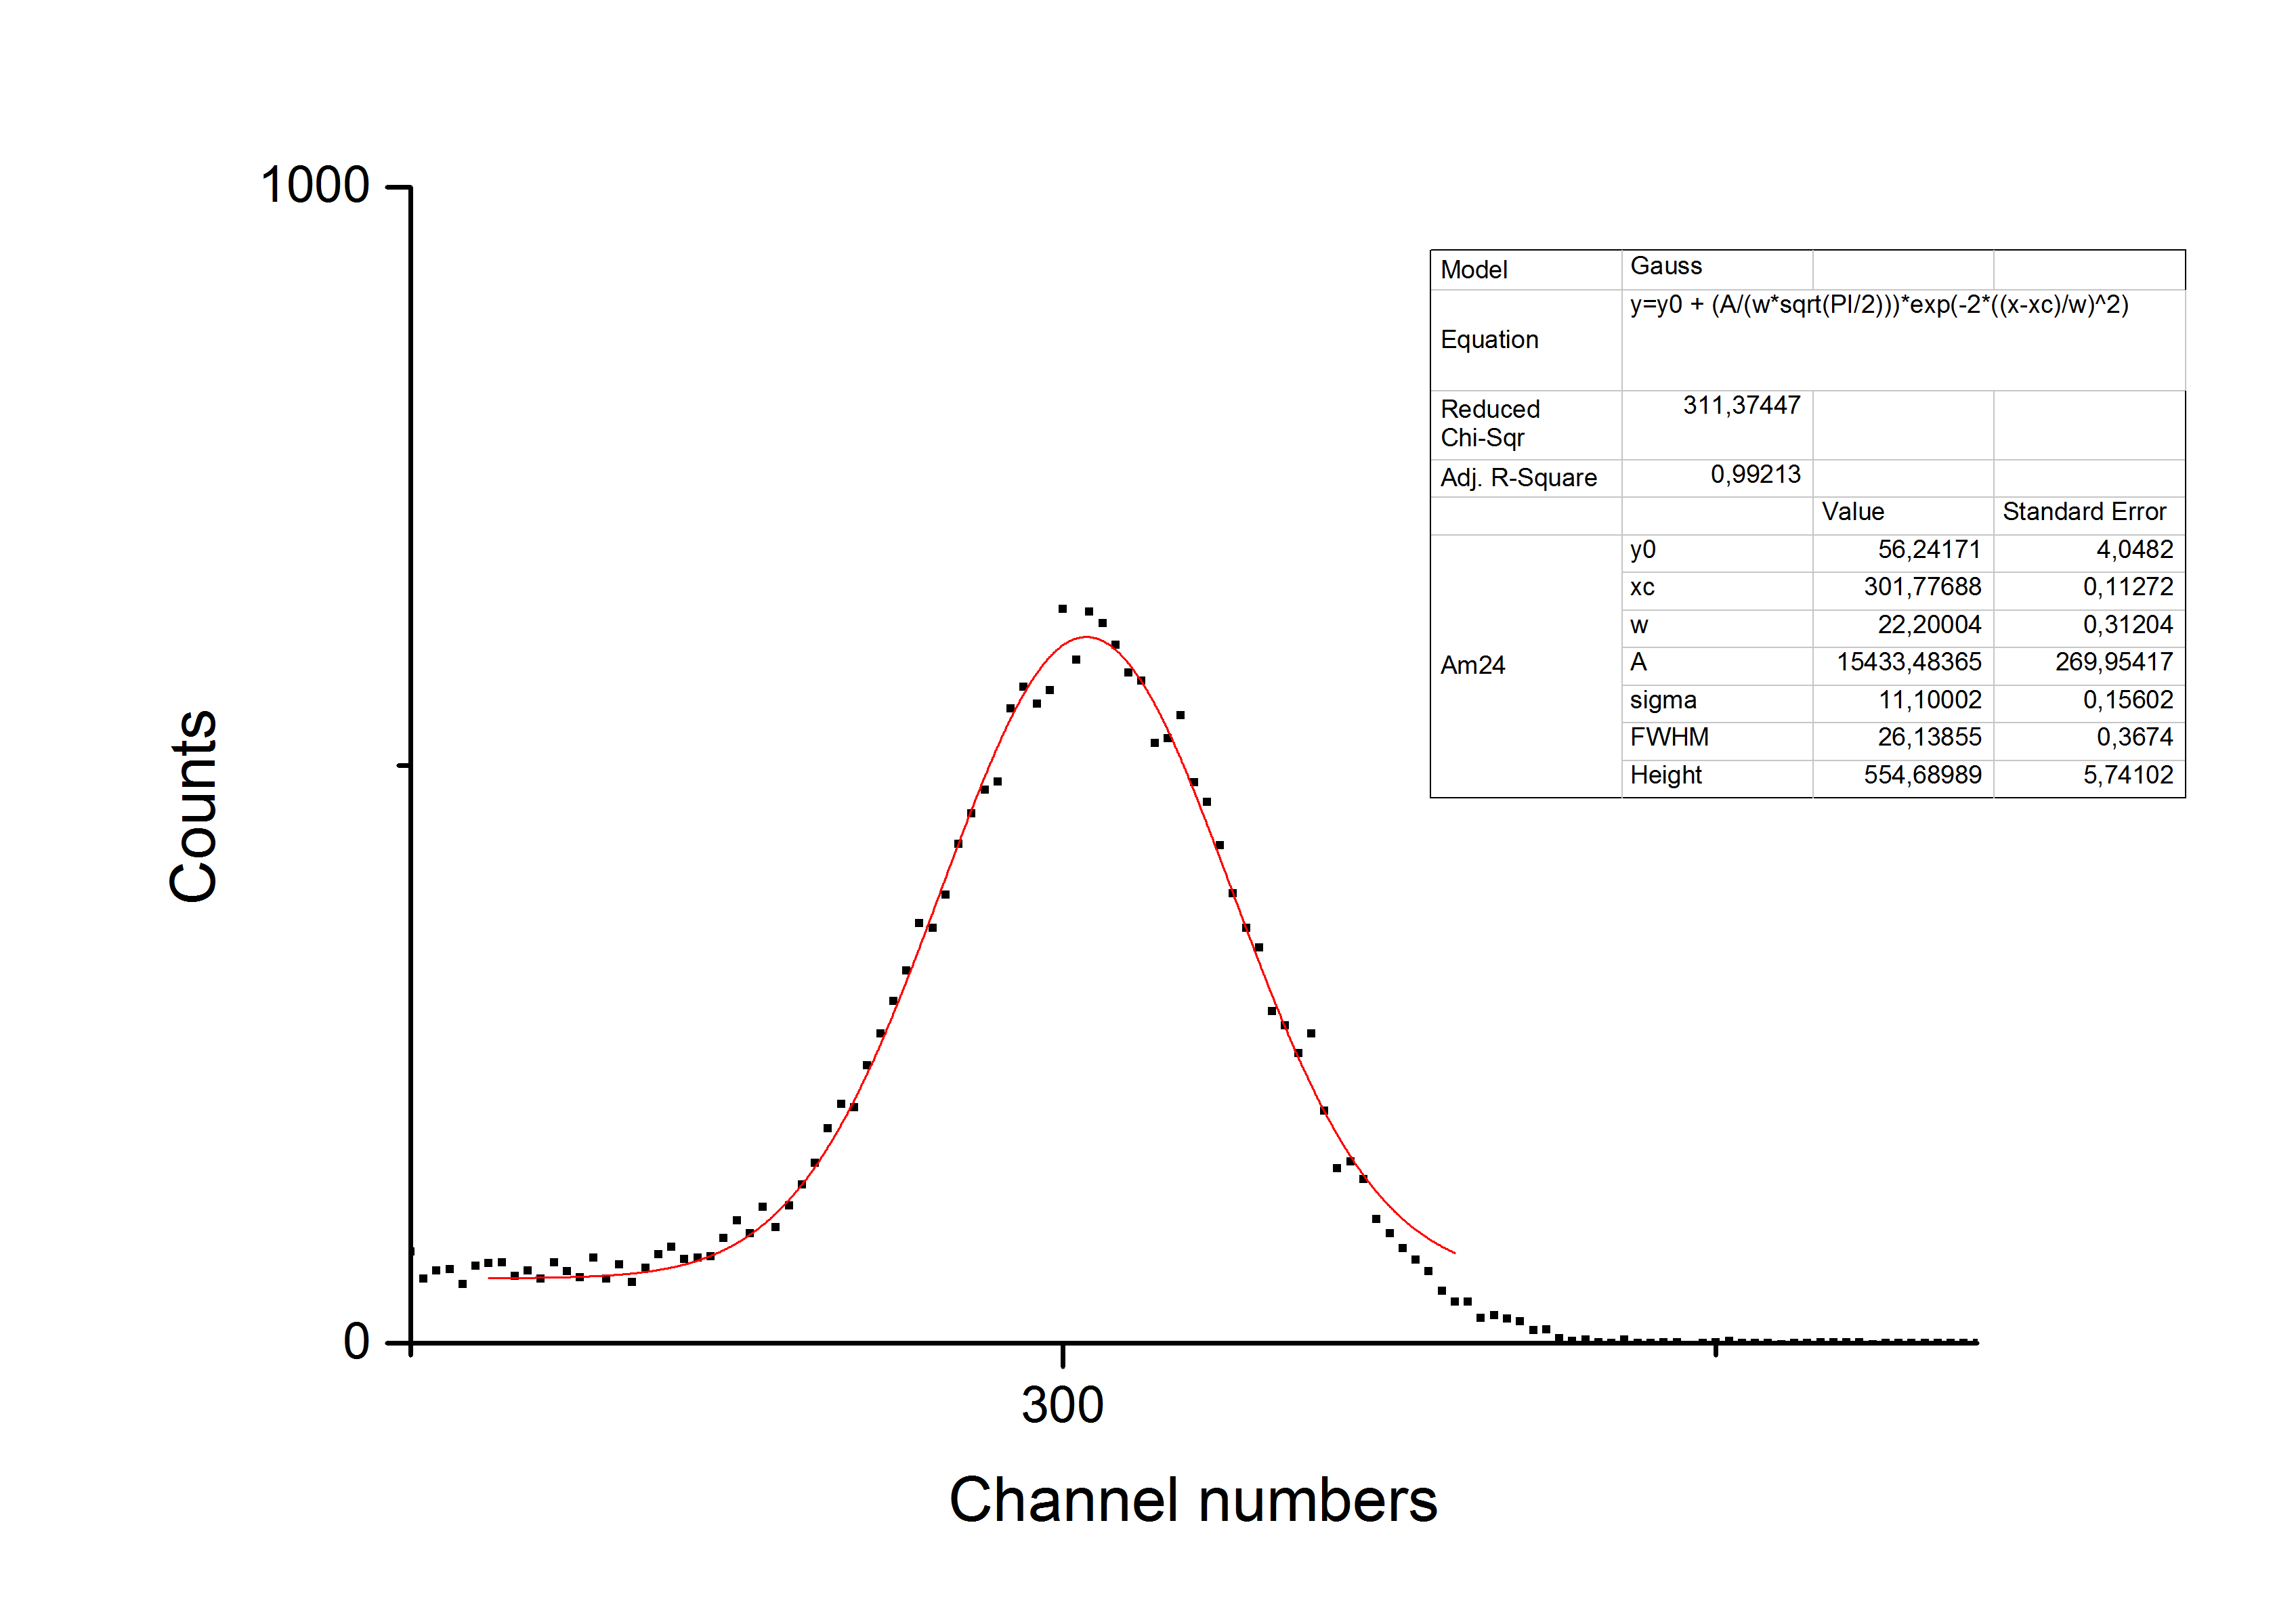
\includegraphics[scale=0.15]{Bilder/Teil3/Am_Si}
\caption{Am with Si-detector}
\label{fig:AmSi}
\end{center}
\end{figure}